\graphicspath{{capitulos/Capitulo2-Definicion-del-problema/recursos/}}


\section{Definición del problema} \label{capitulo:2}

Tal y como se ha indicado anteriormente, el proyecto ABACO pretende automatizar el proceso de creación de un horario de trabajo para los distintos controladores del espacio aéreo de forma que, dada una sectorización de este, todos los sectores puedan ser controlados siguiendo las pautas establecidas por el dominio del problema.

El control del espacio aéreo (también conocido como \gls{ATC}, \textit{\acrlong{ATC}}) es una tarea que se lleva a cabo en todos los aeropuertos con el fin de monitorizar los diferentes aviones que sobrevuelan una determinada zona del cielo, de cara a garantizar la seguridad de sus rutas (lo que se denomina control de ruta), así como de sus aterrizajes (que se llama control de aproximación o de área terminal), encargándose también de las comunicaciones de voz tanto tierra-aire con los pilotos de las aeronaves (vía radio), como tierra-tierra con otros controladores u otro personal de gestión (vía telefónica)~\cite{ENAIRE-web}.
La zona de trabajo de los controladores aéreos se denomina \glspl{Centro de Control}, cuyos puestos de trabajo tienen un aspecto similar al de la \autoref{fig:2:enaire-atc}.

\begin{figure}[htbp]
    \centering
    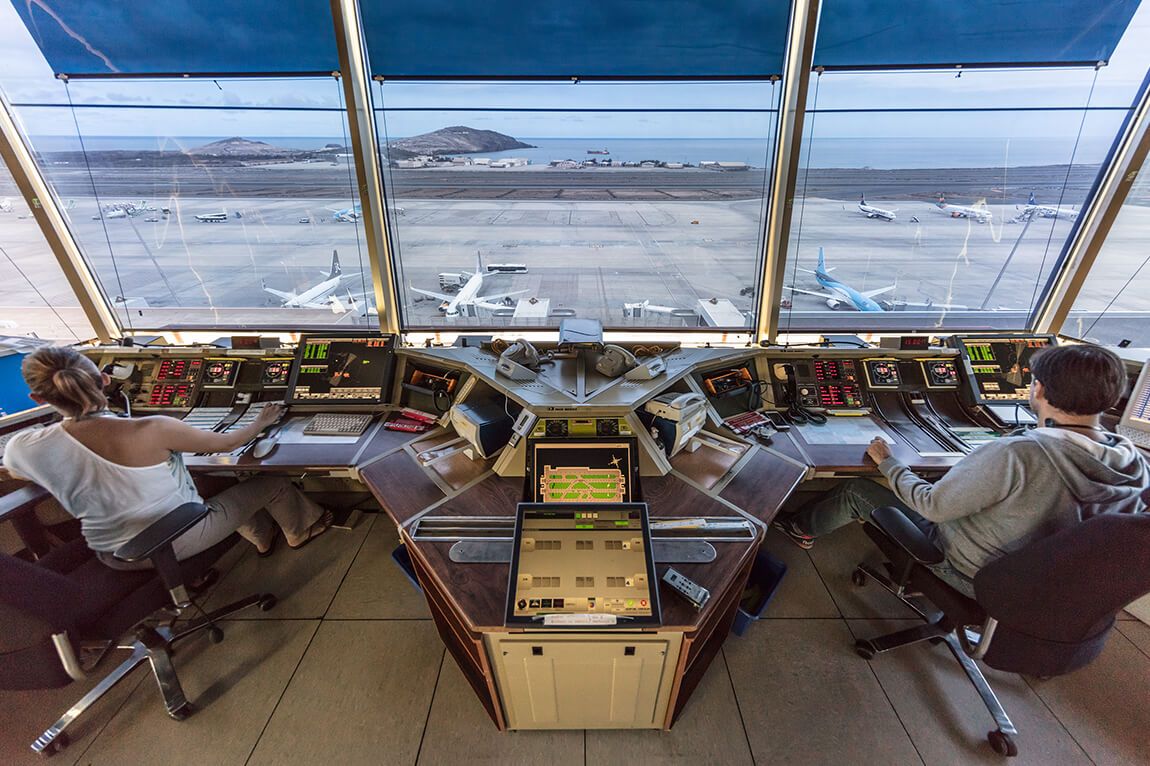
\includegraphics[width=0.7\linewidth]{ENAIRE-ATC}
    \caption[Fotografía de uno de los puestos de control]{Fotografía de uno de los puestos de control, como puede verse 
    está conformado por dos personas. Fuente: 
    \url{https://muia.ml/wzfw8}}
    \label{fig:2:enaire-atc}
\end{figure}


\subsection{Organización del espacio aéreo}
\label{section:2:sectores-y-sectorizacion}
Cada controlador tiene asignado durante un cierto intervalo de tiempo de su turno de trabajo, un sector que debe controlar.
Por ello, en primer lugar, explicaremos brevemente cómo se divide el espacio aéreo del territorio español, cuyo organismo encargado de su gestión es precisamente ENAIRE%
\footnote{\url{https://www.enaire.es/sobre_enaire/conoce_enaire/quienes_somos_ENAIRE}}.
Si bien la realidad es muy compleja, aquí únicamente describiremos una simplificación de la misma, omitiéndose
detalles técnicos de aviación que no son necesarios para la implementación del sistema.

\begin{figure}
	\centering
	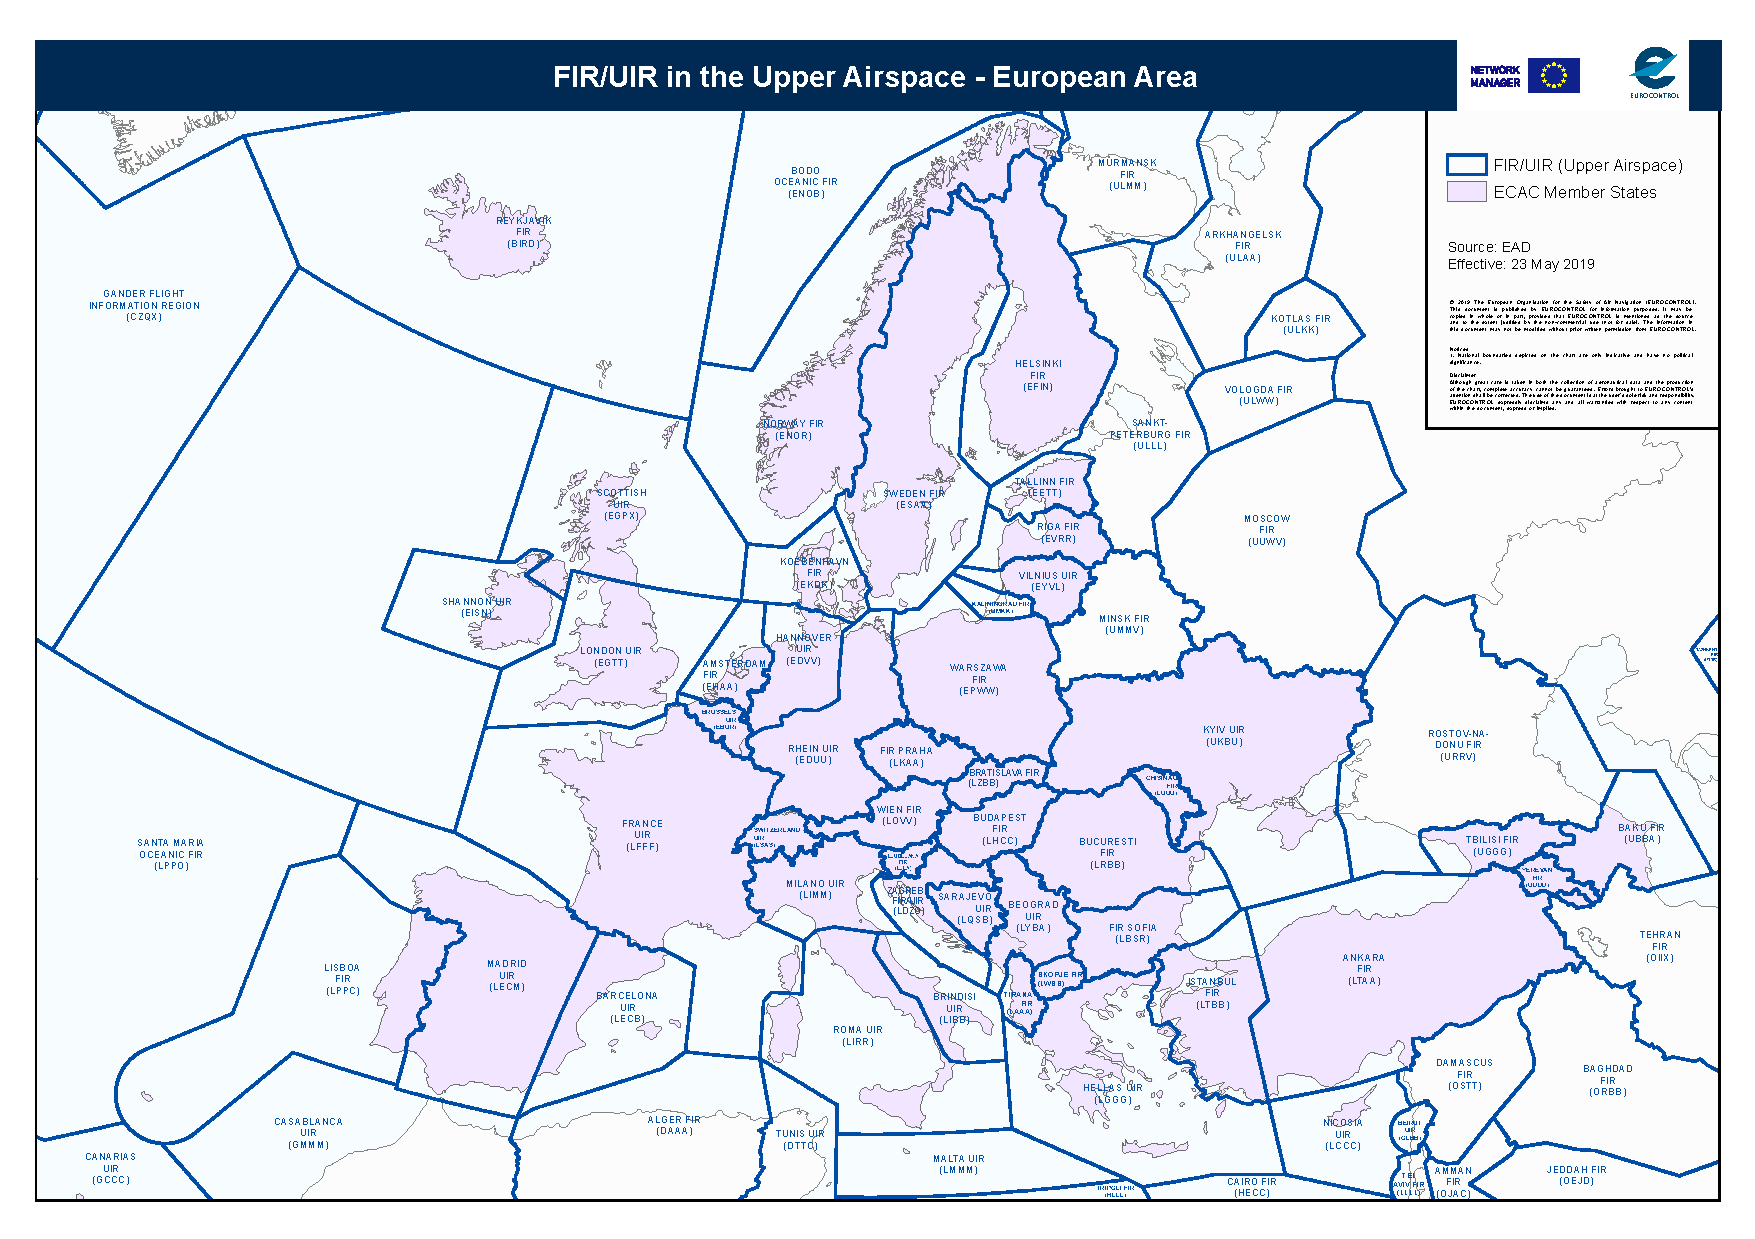
\includegraphics[width=\linewidth]{FIR_europa}
	\caption[FIRs de la zona europea]{FIRs de la zona europea. Fuente: EUROCONTROL}
	\label{fig:2:fireuropa}
\end{figure}

El espacio aéreo mundial se encuentra dividido en \textit{\glspl{FIR}}, áreas del territorio sobre las que se mueven los diferentes aviones de cada compañía aérea de cada país. En la \autoref{fig:2:fireuropa} puede verse gráficamente los límites de cada región.
En el caso de España, podemos ver que tiene control sobre 3 \textit{FIR}s: el de Barcelona, el de Madrid y el de Canarias, sin embargo, a nivel nacional, existen algunas subdivisiones denominadas \textit{Dependencias} (ya que dependen del \textit{FIR} en el que se encuentren), que permiten una mejor gestión del territorio. Las dependencias están constituidas por \glspl{Centro de Control} (uno por cada Dependencia) y Torres de Control. Algunos de ellos aparecerán en los casos reales de prueba del sistema del \autoref{capitulo:5}, así que los enumeramos a continuación:

\begin{figure}
    \centering
    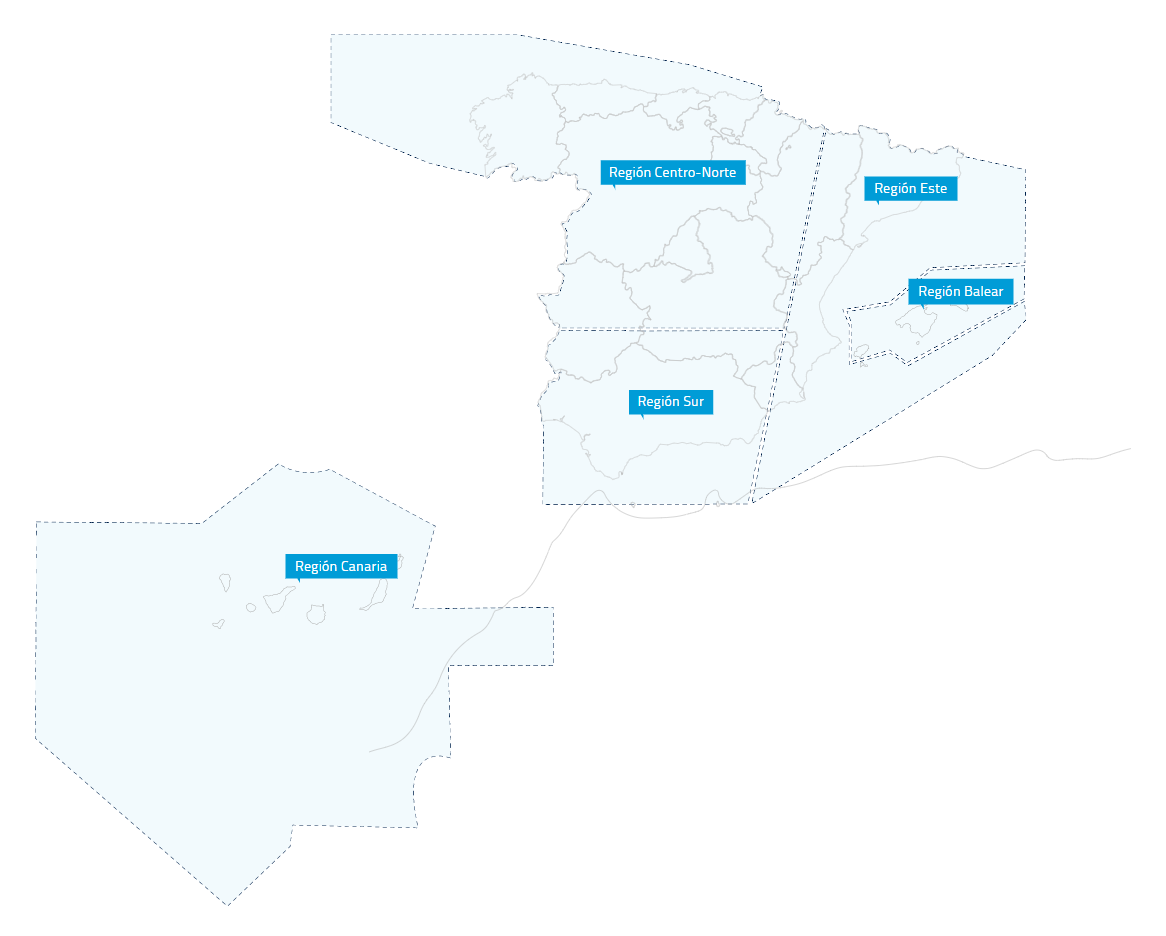
\includegraphics[width=0.7\linewidth]{Division-Espacio-Nacional}
    \caption{Simplificación de la división del espacio aéreo nacional}
    \label{fig:2:regiones}
\end{figure}

\begin{itemize}
    \item Barcelona
    \begin{itemize}
        \item Ruta Este
        \item Ruta Oeste
        \item TMA\footnote{\acrlong{TMA}} ESTE
        \item TMA NORTE
        \item TMA OESTE
    \end{itemize}
    \item Canarias
    \begin{itemize}
        \item ACC App
        \item ACC Ruta
    \end{itemize}
    \item Madrid
    \begin{itemize}
        \item Ruta 1
        \item Ruta 2
        \item TMA NORTE
        \item TMA SUR
    \end{itemize}
    \item Málaga App
    \item Palma TACC
    \item Sevilla TACC
    \item Valencia TACC TMA
\end{itemize}

Cada una de estas Dependencias, está constituida por un cierto número de sectores, que se agrupan de forma que se cubra todo el espacio de la zona, conformando lo que llamaremos una \textit{configuración o sectorización} concreta.
Existen varias configuraciones estandarizadas, de manera que, dado un número de sectores, el espacio aéreo sea cubierto en su totalidad.
Por eso, las sectorizaciones se nombran utilizando dos caracteres: un número y una letra; el número indica precisamente la cantidad de sectores de la configuración, mientras que la letra permite diferenciar entre dos posibles 
configuraciones que emplean el mismo número de sectores.

Por ejemplo, la configuración 3B de la dependencia MADRID Ruta 1 consta de los sectores LECMSAI, LECMBLI y LECMDPI, mientras que una 3D consta de LECMSAN, LECMASI y LECMBDP. En ambos casos se utilizan tres sectores y el espacio cubierto total es equivalente, como puede apreciarse en la \autoref{fig:sectorizacion-3b} y \ref{fig:2:sectorizacion-3d}.
De la misma forma, si utilizamos una configuración 5A, se utilizarían 5 sectores diferentes, pero el espacio aéreo a controlar sería nuevamente equivalente, como se aprecia en la \autoref{fig:2:sectorizacion-5a}.
Nótese además, que los sectores LECMSAN (amarillo) y LECMASI (verde) son los mismo que los de la sectorización 3D (\autoref{fig:2:sectorizacion-3d}) pero el sector LECMBDP (azul) se ha dividido o \textit{abierto} en los sectores LECMBLI, LECMDGI y LECMPAI.

\begin{figure}[htbp]
    \centering
    \begin{subfigure}{\linewidth}
        \centering
        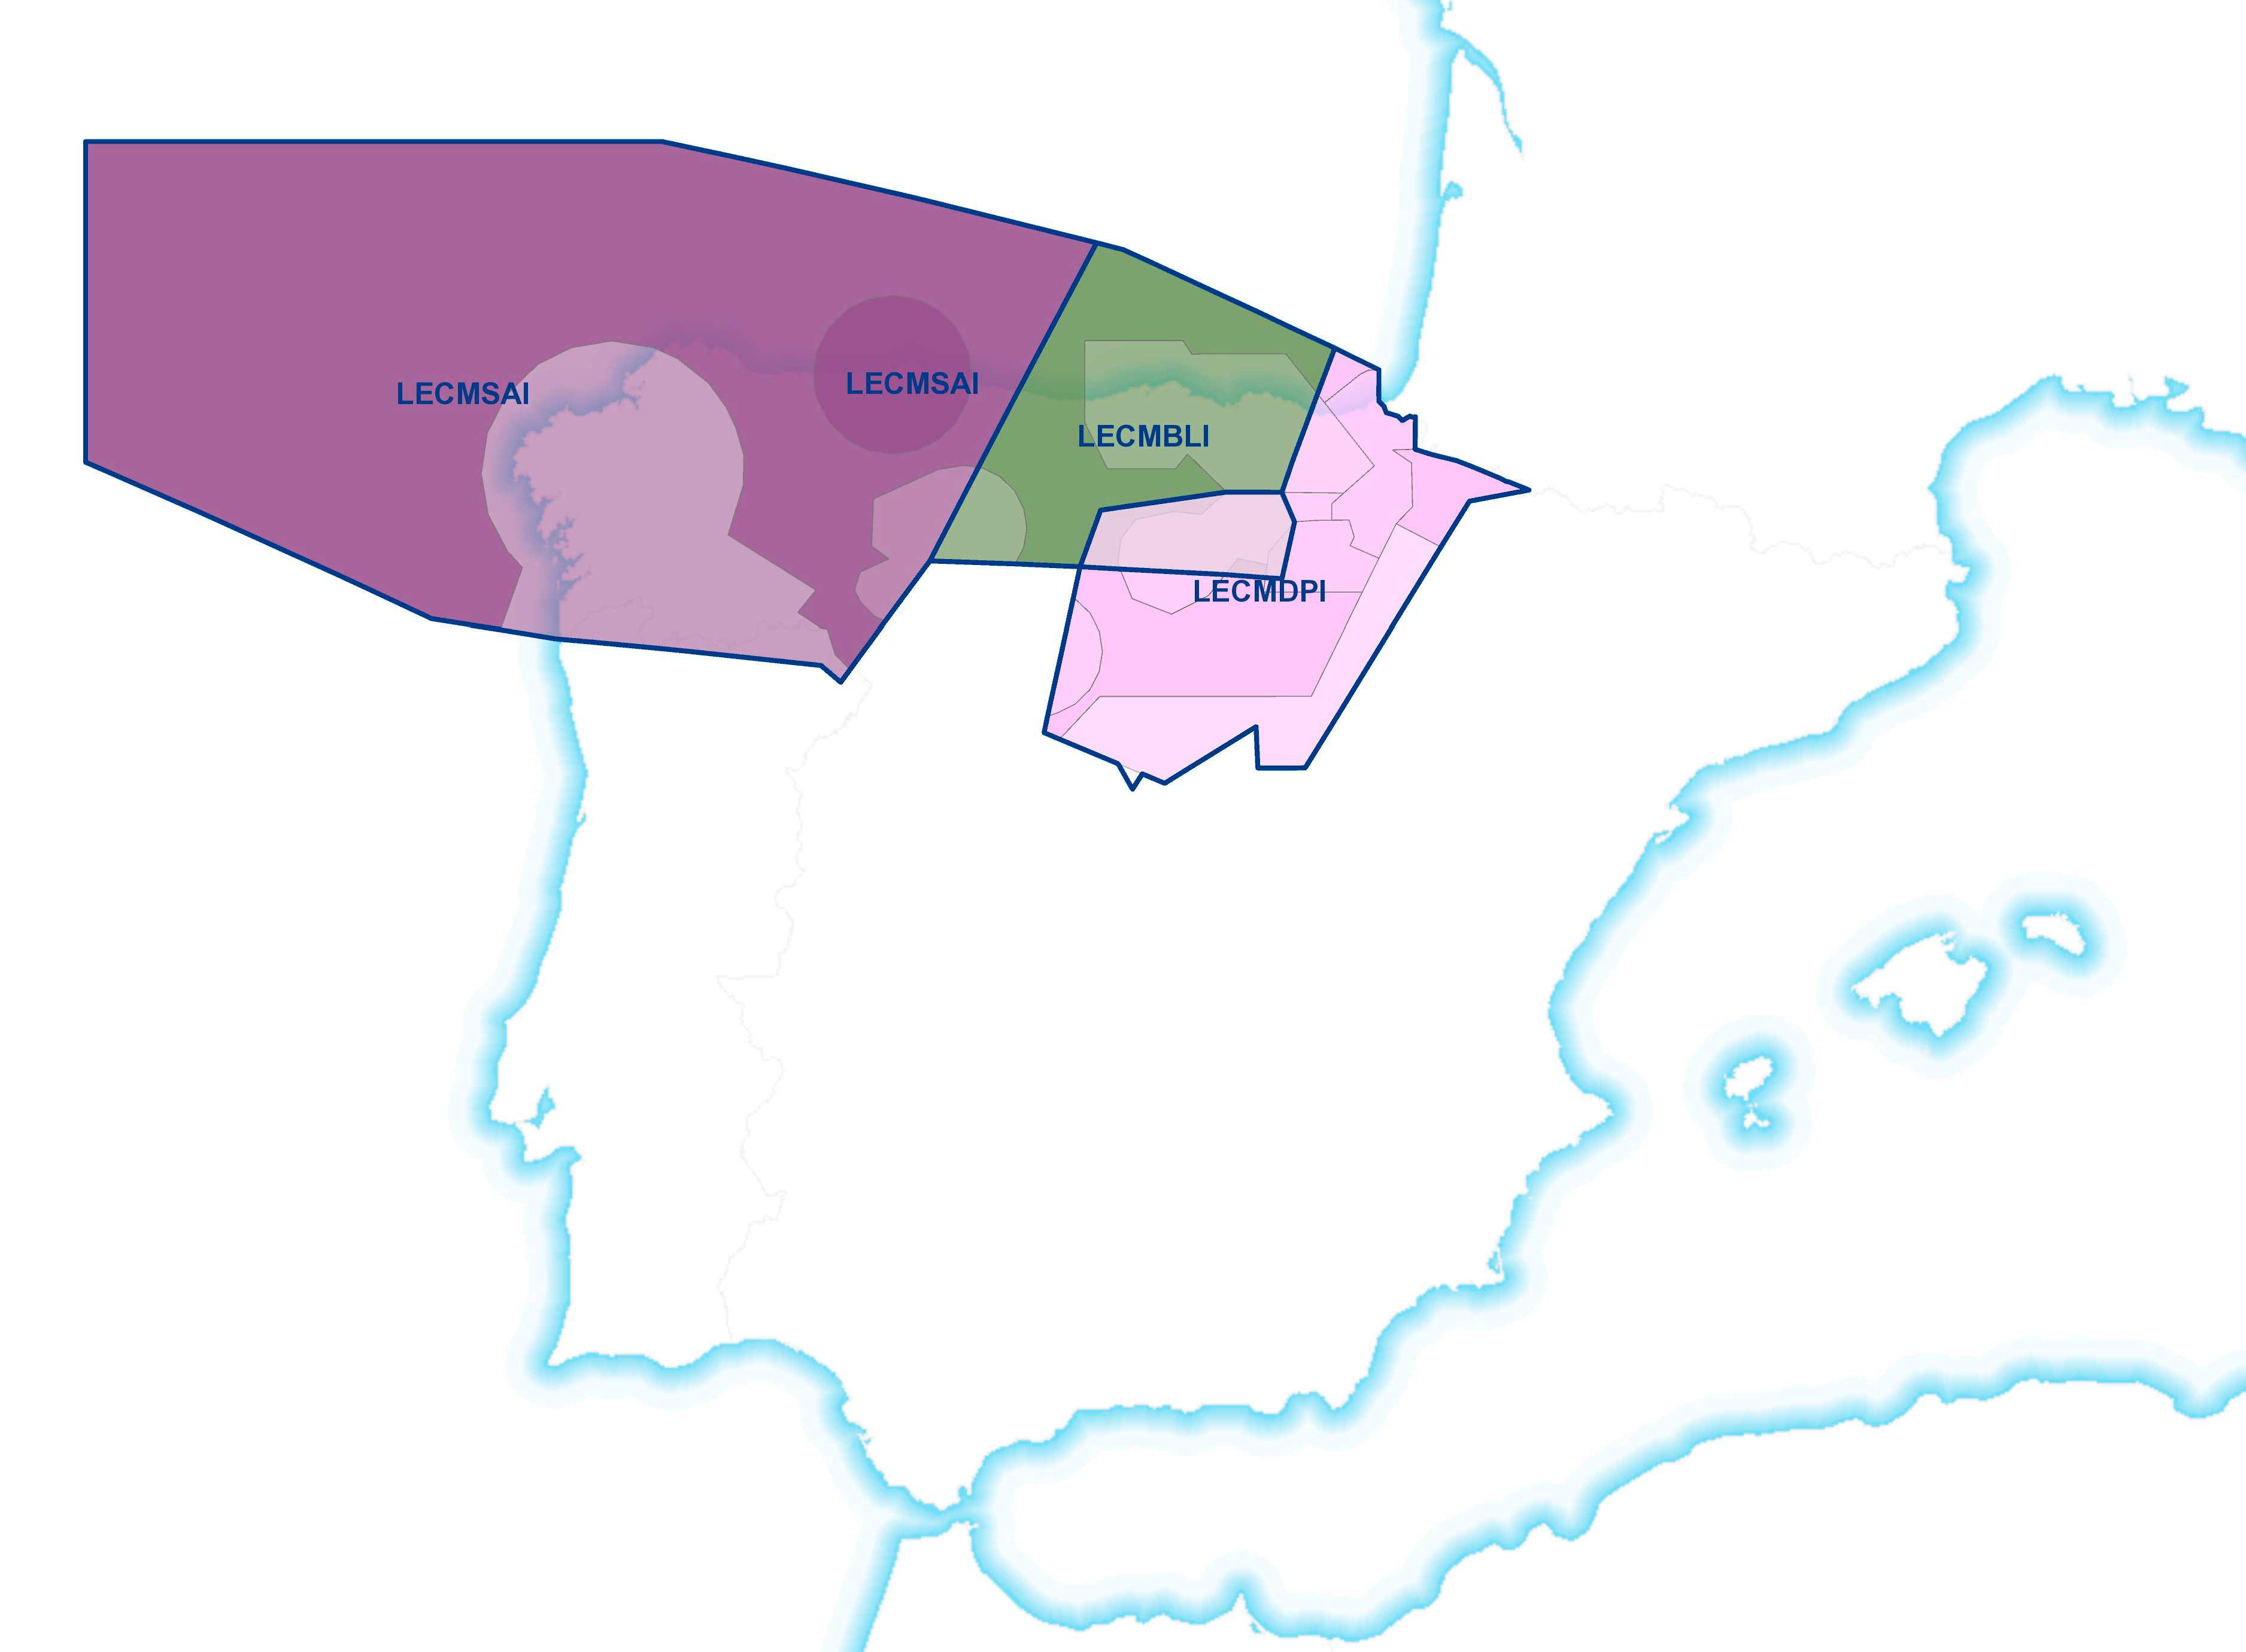
\includegraphics[width=0.58\linewidth]{sectorizacion-3B}
        \caption{sectorización 3B\linebreak}
        \label{fig:sectorizacion-3b}
    \end{subfigure}

    \begin{subfigure}{\linewidth}
        \centering
        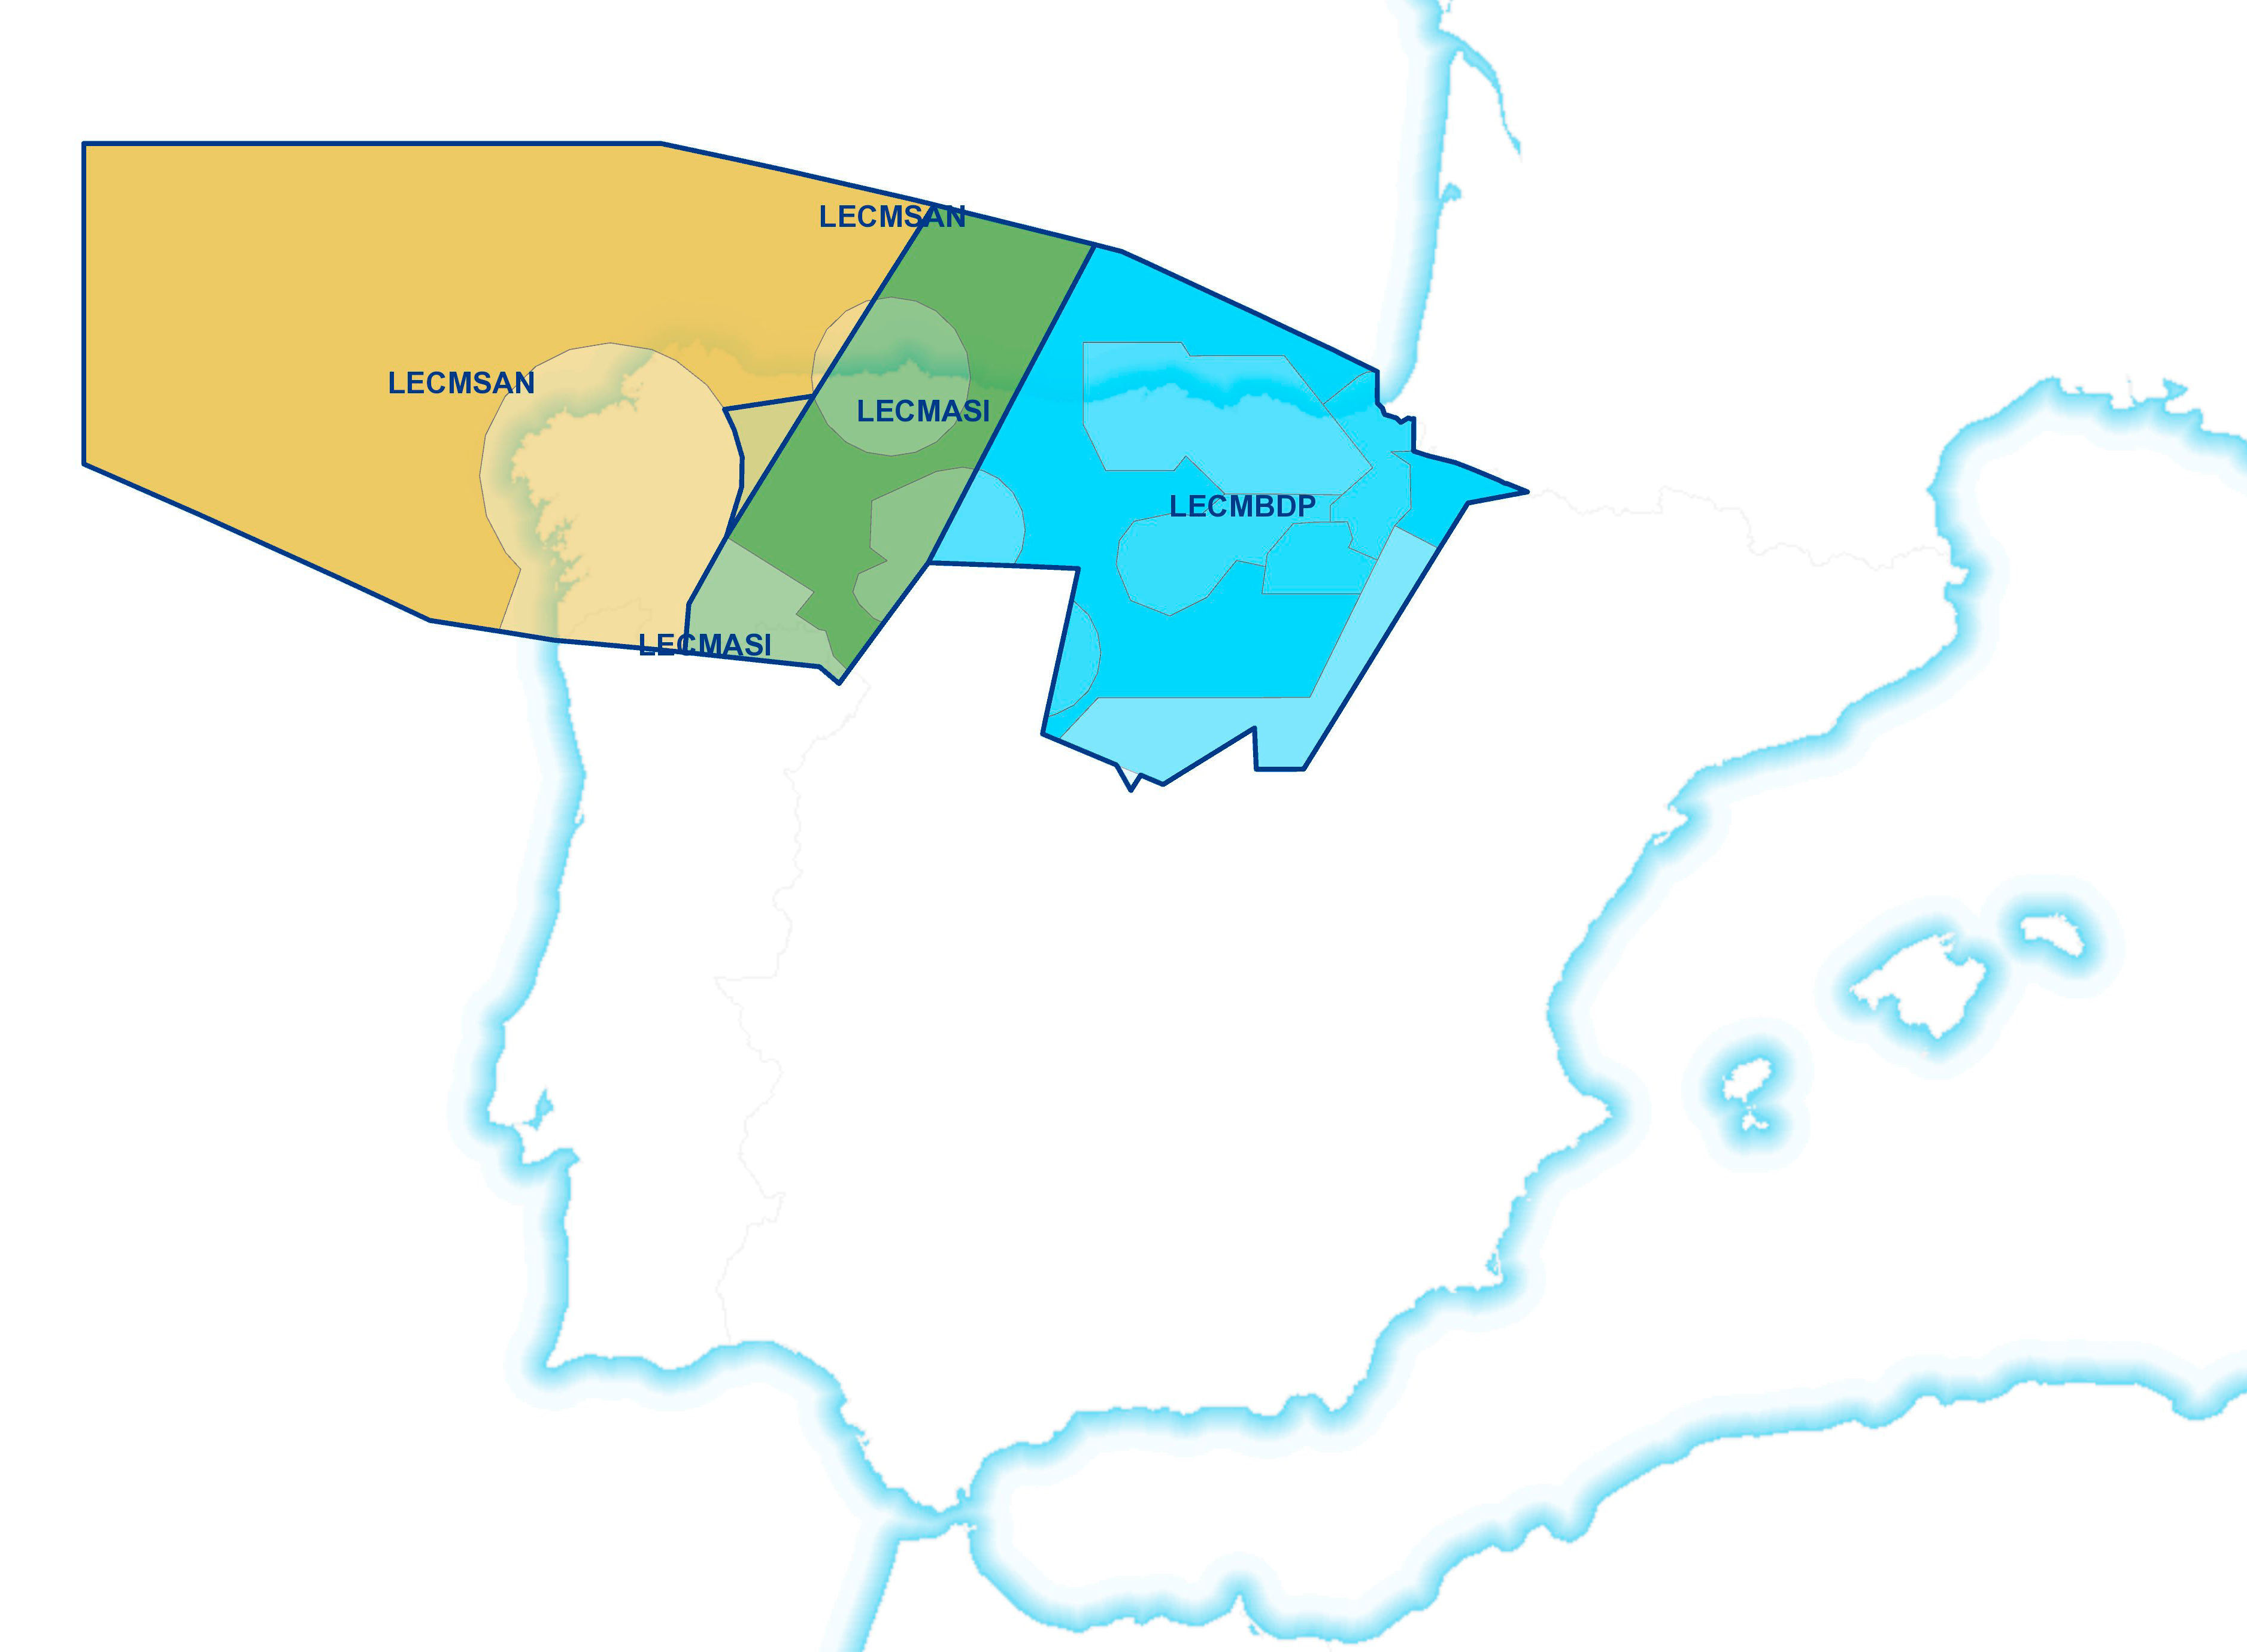
\includegraphics[width=0.58\linewidth]{sectorizacion-3D}
        \caption{sectorización 3D\linebreak}
        \label{fig:2:sectorizacion-3d}
    \end{subfigure}

    \begin{subfigure}{\linewidth}
        \centering
        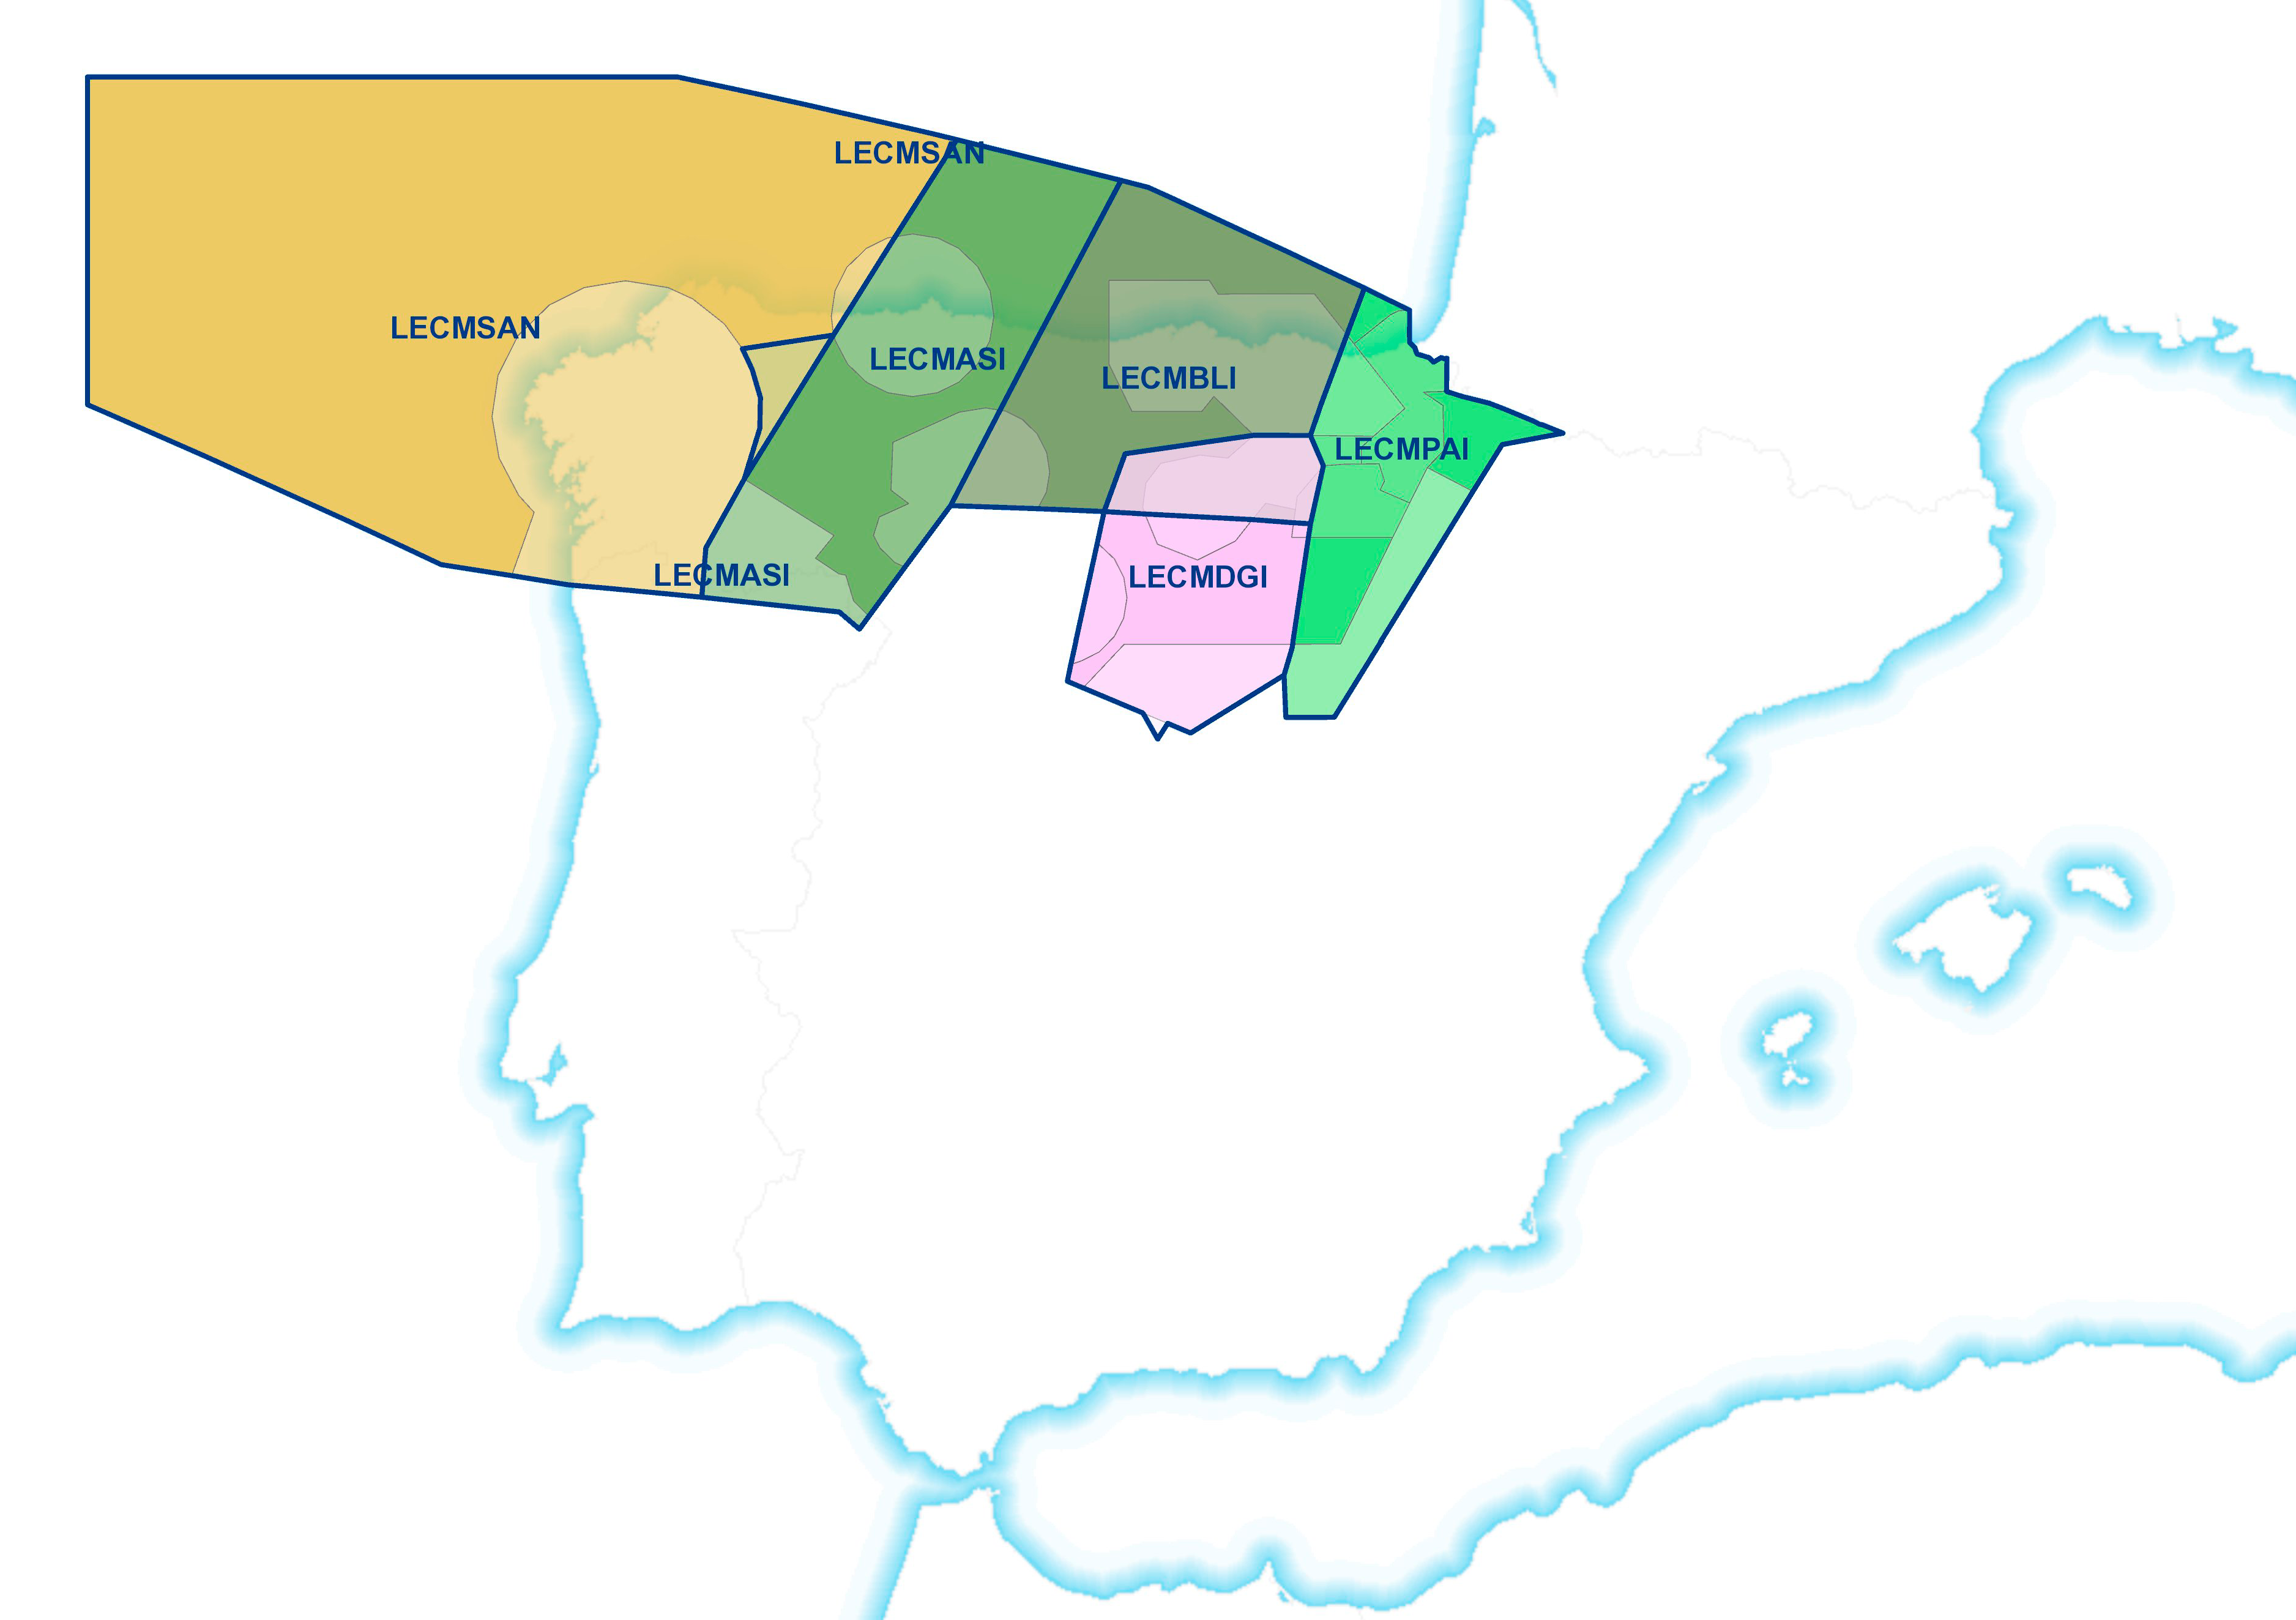
\includegraphics[width=0.58\linewidth]{sectorizacion-5A}
        \caption{sectorización 5A}
        \label{fig:2:sectorizacion-5a}
    \end{subfigure}

    \caption[Ejemplo de sectorización 3B y 3D de la dependencia MADRID Ruta 1]{Ejemplo de comparativa de una 
    sectorización 3B y 3D 
    de la dependencia MADRID Ruta 1}
    \label{fig:2:comparativa3B-3D}
\end{figure}


Cuando cambiamos de una configuración de partida a otra, nos encontramos 2 posibles situaciones: que pasemos de una sectorización con un menor número de sectores a otra con mayor (como en el ejemplo anterior) donde se \textit{abrirán} sectores; o por el contrario que pasemos de una sectorización con un mayor número de sectores a otra menor (por ejemplo, el caso contrario: de una 5A a una 3D) donde se \textit{cerrarán} sectores, pero como hemos visto, algunos serán comunes y no sufrirán cambio. 
Teniendo siempre en cuenta que se ha de controlar la totalidad de espacio aéreo de la zona, sin superposiciones o espacios sin controlar, por ello en algunos casos un mayor número de sectores se ve afectado, pudiendo tanto abrirse como cerrarse diferentes sectores para adecuarse a la nueva configuración.

Existen dos tipos de sectores: Ruta y Aproximación (APP), que tienen que ver con el tipo de tareas que los 
controladores llevan a cabo.
Los sectores de tipo Ruta precisan de tareas de control de ruta: garantizar la seguridad en las rutas de las naves aéreas; mientras que los sectores de tipo Aproximación precisan de tareas de aproximación o de área terminal: principalmente la gestión de los aterrizajes en el aeropuerto.

El siguiente concepto importante es el de afinidad entre sectores. Sin entrar en demasiado detalle, la unidad mínima de división del espacio aéreo son los volúmenes, de esta forma los sectores cubrirán un determinado número de volúmenes.
Pues diremos que dos sectores \textit{son afines entre sí} si comparten al menos un volumen entre sí. Para saber si dos sectores son afines, utilizaremos la llamada \textit{matriz de afinidad} que, si bien puede ser construida manualmente, en nuestro caso será tratada como un input del sistema para ahorrar tiempo innecesario de cómputo, pues es constante para cada dependencia (en el Capítulo XXX se muestra un ejemplo). %TODO referencia!!

Por último, resta introducir el concepto de \textit{núcleo}. Un núcleo no es más que una agrupación de alto nivel de varios sectores, pudiendo un sector pertenecer a varios núcleos (relación N a N). El uso de los núcleos facilita la gestión de la acreditación los controladores aéreos, pudiendo estos controlar únicamente un determinado núcleo (véase Requisito XXX). %TODO referencia


\subsection{Gestión de tráfico aéreo}
La gestión del tráfico aéreo (\gls{ATC}) se desempeña en las salas de control por un conjunto de trabajadores 
llamados controladores aéreos. Los controladores trabajan a lo largo de un turno de una duración determinada, que puede ser de Mañana, Tarde o Noche, con la peculiaridad de que los de Mañana y Tarde pueden ser de tipo Largo o Corto. 
Cuando el turno es Largo quiere decir que se toma parte del turno de noche, extendiendo así el periodo laboral (se ilustra un ejemplo en la \autoref{fig:2:tipos-turnos}). Cada \acrlong{Centro de Control} tiene sus propios horarios predefinidos para cada uno de los turnos.

\begin{figure}
	\centering
	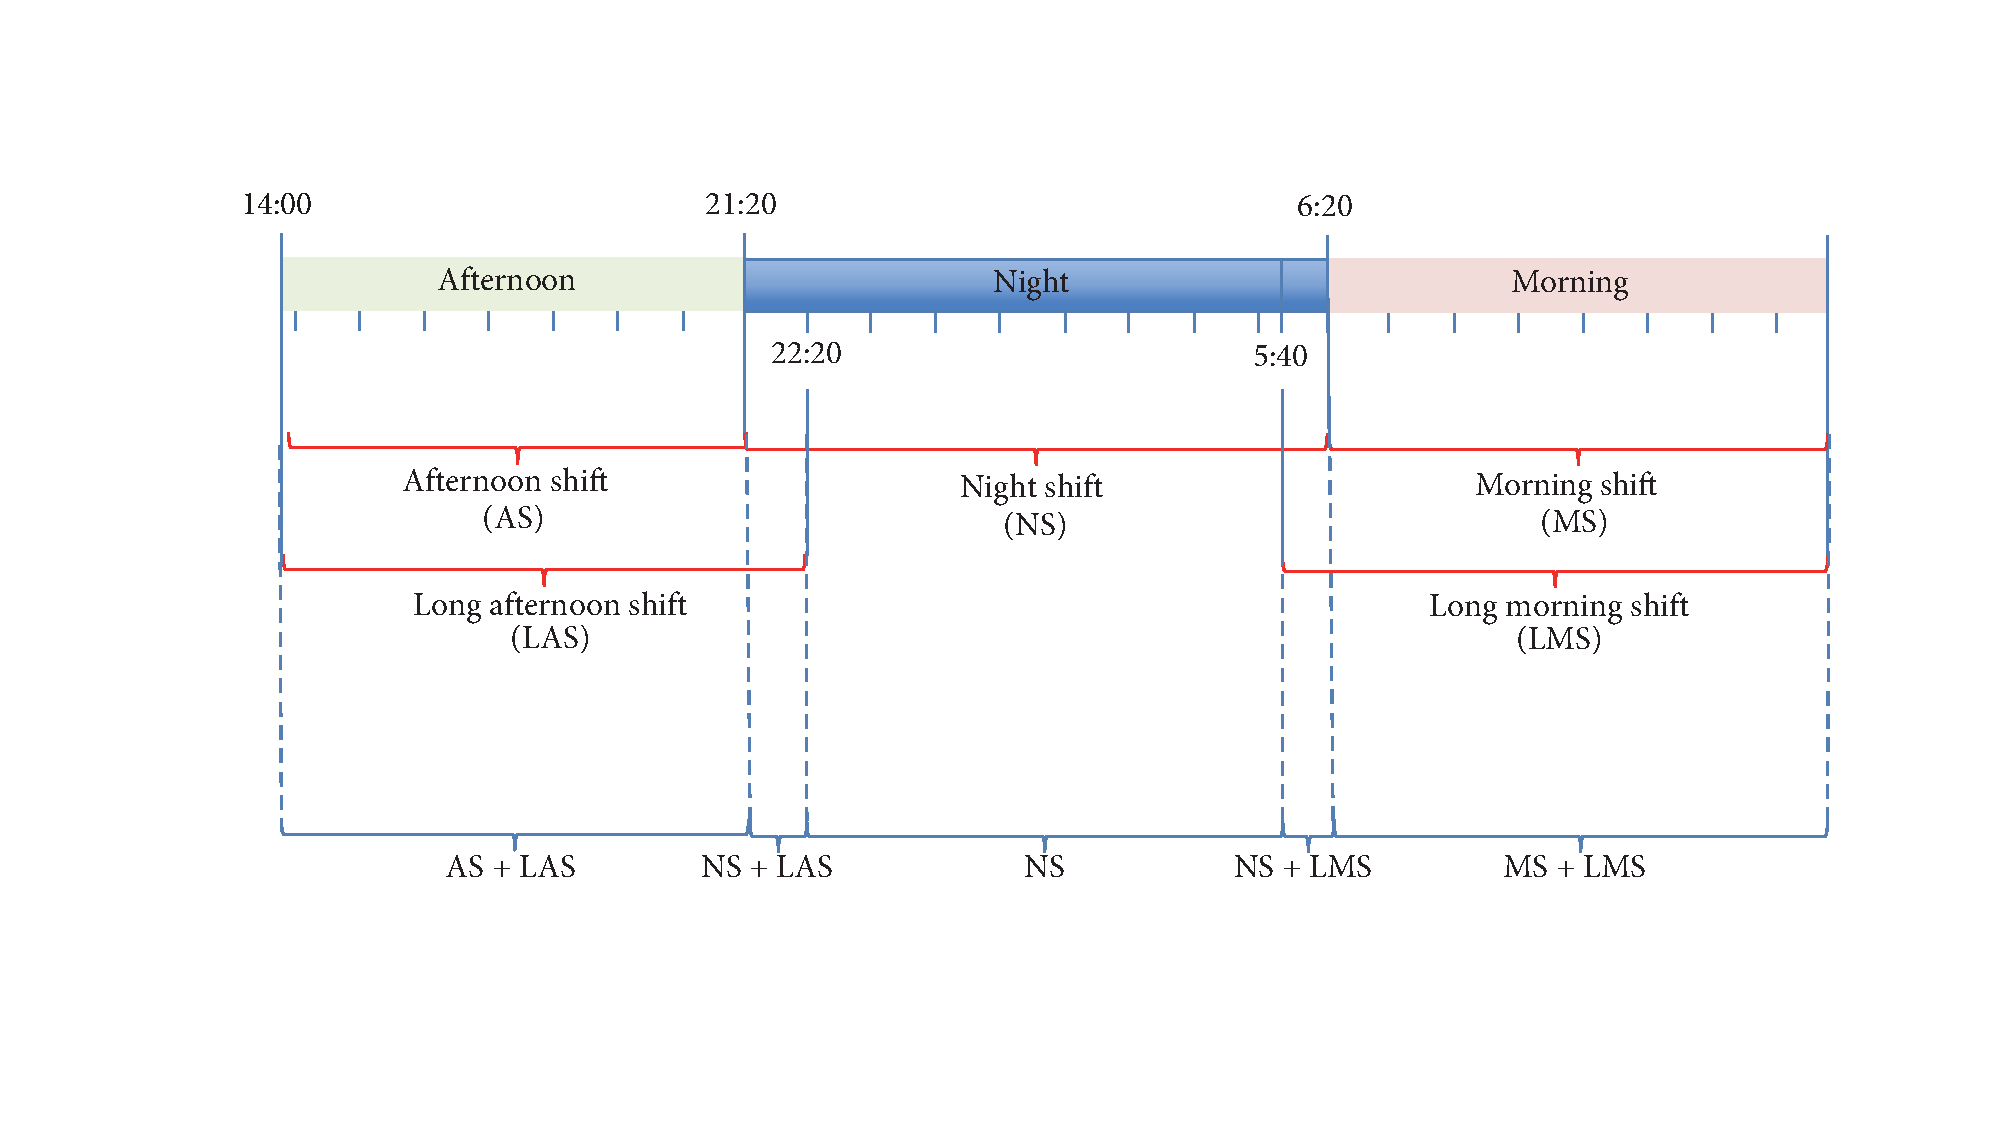
\includegraphics[width=\linewidth]{tipos-turnos}
	\caption[Esquema que representa los tipos de turnos]{Esquema que representa los tipos de turnos. 
	Fuente:~\cite{articulo1}}
	\label{fig:2:tipos-turnos}
\end{figure}

Por otro lado, en cada puesto de control debe haber dos controladores, cada uno en una posición diferente: 
\textit{ejecutivo} y \textit{planificador}. El controlador en posición planificador es responsable de anticiparse a posibles problemas y avisar al otro controlador (en posición ejecutivo) antes de que éstos lleguen a producirse. Por su parte, el ejecutivo es quien debe llevar a cabo la tarea principal, así como solucionar los conflictos que el planificador le comunique. La fotografía de la \autoref{fig:2:enaire-atc} muestra cómo es uno de estos puestos de trabajo, con un controlador de cada tipo.

Como ya se comentó en el apartado anterior, cada controlador tiene una acreditación que le permite controlar un \gls{Nucleo} específico y, por ende, únicamente podrá trabajar en puestos que impliquen el control del 
tráfico aéreo de un determinado conjunto de sectores, lo que equivaldría a una sección específica del espacio aéreo total.

Adicionalmente, en vista de las diferentes tareas a realizar por los controladores en función del tipo de sectores, parece lógico pensar que exista acreditación adicional, que aumenta el nivel de restricción de los sectores que puede controlar en función del tipo que estos sean. Por ello, hay dos tipos de acreditaciones, que tienen el nombre de PTD y CON. Los controladores con acreditación CON, únicamente podrán controlar los sectores de tipo Ruta, mientras que los de tipo PTD pueden controlar tanto Ruta como Aproximación (véase \autoref{table:2:acreditaciones}).

%\begin{table}[h]
%	\centering
%	\caption[Tipos de sectores según la acreditación del controlador]{Tipos de sectores que se pueden controlar según el tipo de acreditación de un controlador}
%	\begin{tabular}{lcc}
%		\hline
%		\textbf{Tipo acreditación} & \textbf{Sectores tipo Ruta} & \textbf{Sectores tipo Aproximación} \\ \hline
%		PTD                        &        $\checkmark$         &            $\checkmark$             \\
%		CON                        &        $\checkmark$         &                                     \\ \hline
%	\end{tabular}
%	\label{table:2:acreditaciones}
%\end{table}


\begin{table}[h]
	\centering
	\caption[Tipos de sectores según la acreditación del controlador]{Tipos de sectores que se pueden controlar según el tipo de acreditación de un controlador}
	\begin{tabular}{lcc}
		\hline
		\textbf{Tipo acreditación} & \textbf{PTD} & \textbf{CON} \\ \hline
		Sectores tipo Ruta         & $\checkmark$ & $\checkmark$ \\
		Sectores tipo Aproximación & $\checkmark$ &              \\ \hline
	\end{tabular}
	\label{table:2:acreditaciones}
\end{table}
%
%\NOTE{Elegir una de las tablas}

La configuración de sectores en cada instante de tiempo puede variar en función del flujo del tráfico aéreo zonal, por lo que no puede conocerse con exactitud previamente. No obstante, puede ser predicho con antelación, de manera que se pueda realizar la asignación de controladores a puestos previamente.
Es en este punto donde diverge el sistema existente con el propuesto en la presente tesis. 
Más detalladamente en la \autoref{capitulo:2:detalles-sistema}.

Supongamos el ejemplo de la \autoref{fig:2:ejemplo-apertura-sectorizaciones}, en la que se muestra una posible sectorización predicha con antelación por el personal del aeropuerto. Podemos apreciar los conceptos definidos anteriormente: el turno de trabajo de mañana, que para este \gls{Centro de Control} comienza y finaliza a las 7:30 y 15:00 horas, respectivamente; también las sectorizaciones de cada uno de los núcleos afectados (en este caso son dos), en el caso del núcleo \textit{Barcelona Ruta Oeste} tenemos una configuración 3D para todo el turno, mientras que en el caso del otro, \textit{Barcelona Ruta Este}, ocurre un desdoblamiento de un 5A a una 6C (uno de los sectores de la 5A se subdivide en dos; otros se cierran y son sustituidos por otros de forma que no haya superposición entre ellos).

\begin{figure}[htbp]
	\centering
	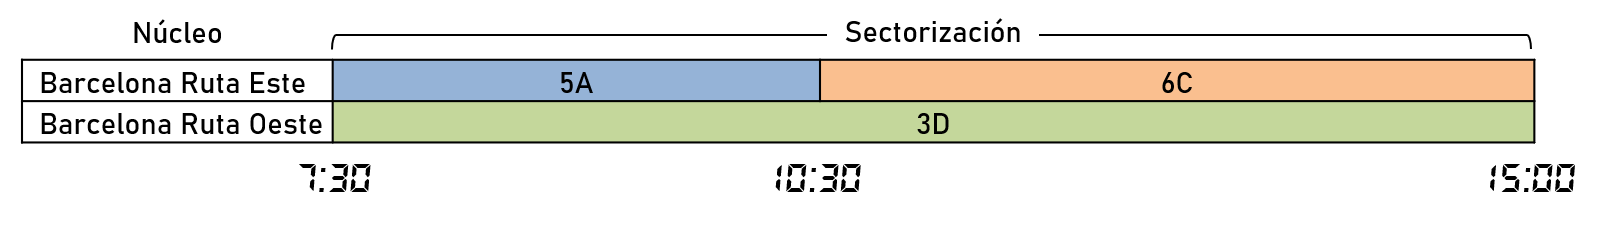
\includegraphics[width=\linewidth]{ejemplo-apertura-sectorizaciones}
	\caption{Ejemplo de sectorización para un turno de un día concreto}
	\label{fig:2:ejemplo-apertura-sectorizaciones}
\end{figure}

\subsection{El sistema \legacy{}}
\label{capitulo:2:detalles-sistema}
Llegados a este punto es importante diferenciar la naturaleza de sendos sistemas, de planificación y táctico, pues si bien tienen en común el dominio del problema presentado en apartados previos, son muy diferentes en cuanto a su naturaleza.

El sistema planteado y resuelto anteriormente por el grupo de investigación de análisis de decisiones y estadística\footnote{\url{http://dia.fi.upm.es/dasg/}} y del que reutilizamos partes de la funcionalidad (en adelante \texttt{Legacy}) resolvía el problema de asignación de controladores con antelación previa, por lo que los requerimientos de software relativos a la eficiencia no eran estrictos, esto es, el tiempo no era un factor crítico (si bien importante en todo sistema de optimización inteligente). El sistema podía permanecer en segundo plano durante horas para lograr alcanzar una solución válida (ya sea una óptima o simplemente factible), no obstante, para el nuevo sistema sucede lo contrario: 
el tiempo es un factor vital, el problema no se está resolviendo con antelación sino al momento de surgir una contingencia imprevista en la planificación, por lo tanto, es necesario reorganizar todo el plan para adecuarlo a dicha contingencia, que puede ser de varios tipos, aunque para el presente trabajo hemos considerado los dos más urgentes e importantes: baja inesperada de uno de los controladores (con posible reincorporación) y cambio imprevisto de la sectorización en un instante dado. 
El personal del centro normalmente tendría conocimiento de las contingencias unos 10 minutos antes de producirse, por lo que el problema táctico debe resolverse en tiempo real, idealmente antes de que la incidencia se produzca y poder reorganizar a los controladores de la forma más amena posible.
Por todo ello, no solamente cambia la naturaleza del sistema, sino también los objetivos del mismo.

El enfoque llevado a cabo en el nuevo sistema para su resolución sigue la misma línea de investigación que los anteriores, una metaheurística como aplicación directa de la Inteligencia Artificial en el ámbito de la optimización multiobjetivo.
Los antecedentes del proyecto resuelven el problema de planificación mediante dos metaheurísticas diferentes: \gls{SA} y \gls{VNS}, ambas de naturaleza muy diferente. 
Esta serie de proyectos anteriores llegó a su culminación mediante una publicación en la revista \textit{Mathematical Problems in Engineering}~\cite{articulo1} y posteriormente otra en \textit{Mathematics -- Open Access Journal}~\cite{articulo2}. 
En este último se comparan resultados de sendas metaheurísticas, donde puede apreciarse que el SA es superior en casi todos los casos, aunque en tiempo de ejecución el VNS le supera, salvo en dos instancias. Por ello, en este caso en el que el tiempo es crucial, parece prometedora la idea del VNS para este nuevo sistema. 

La metodología propuesta (véase \autoref{capitulo:3}) para este nuevo sistema es completamente diferente a la propuesta por Tello et al. en~\cite{articulo1}, no obstante, existen conceptos y subprocesos equivalentes en ambos. 
A lo largo de las próximas secciones subrayaremos otras diferencias entre ambos sistemas más concretas en cuanto a implementación y a la metodología.

Finalmente, es importante destacar que el origen de ambos proyectos pretende automatizar el proceso de planificación que actualmente llevan a cabo manualmente, y que el sistema \legacy{} será utilizado como herramienta para generar planificaciones diarias, por lo que el sistema aquí presentado podrá utilizar el formato de salida del anterior como una entrada (más detalles en el \autoref{capitulo:3}) 



% TODO: reeler y adecuar, llamar regiones en lugar de dependencias y comentar los tipos de estaciones (ACC o torre) y 
%despues listar las diferentes que hay (la lista de arriba)
